\section*{Method}

I used a local descent method with backtracking line search for all three simple problems.
At each iteration, the optimizer computes the gradient, forms the normalized descent
direction
\[
    d = -\frac{\nabla f(x)}{\|\nabla f(x)\|},
\]
Then, the method uses backtracking line search to choose the step size if:
\[
f(x^{(k+1)})\leq f(x^{(k)})+\beta \alpha \nabla_{d^{(k)}} f(x^{(k)})
\]
with initial params $\alpha=1.0, \beta=1e-4$ and a constant factor $p=0.5$ to decrease $\alpha$ until sufficient decrease is satisfied. 

The update then is
\[
    x_{k+1} = x_k + \alpha_k d_k.
\]

The implementation checks the remaining budget before taking a new step.

\section*{Local Test Results}

Current implementation beat random search at the following rates:

\begin{itemize}[leftmargin=1.5em]
    \item \texttt{simple1}: 71.8\%
    \item \texttt{simple2}: 96.6.0\%
    \item \texttt{simple3}: 99.0\%
\end{itemize}

This method is simple and reliable on the provided test functions. It performs best on
Himmelblau's and Powell's functions.

The performance on \texttt{simple1} could be due to Rosenbrock's function being 
more difficult for normalized gradient descent because the optimum lies inside a
curved valley. The method tends to zig-zag across that valley, and with only
20 evaluations available, there is limited budget to correct the direction and take
many productive steps.

\section*{Rosenbrock Path}

\begin{figure}[H]
    \centering
    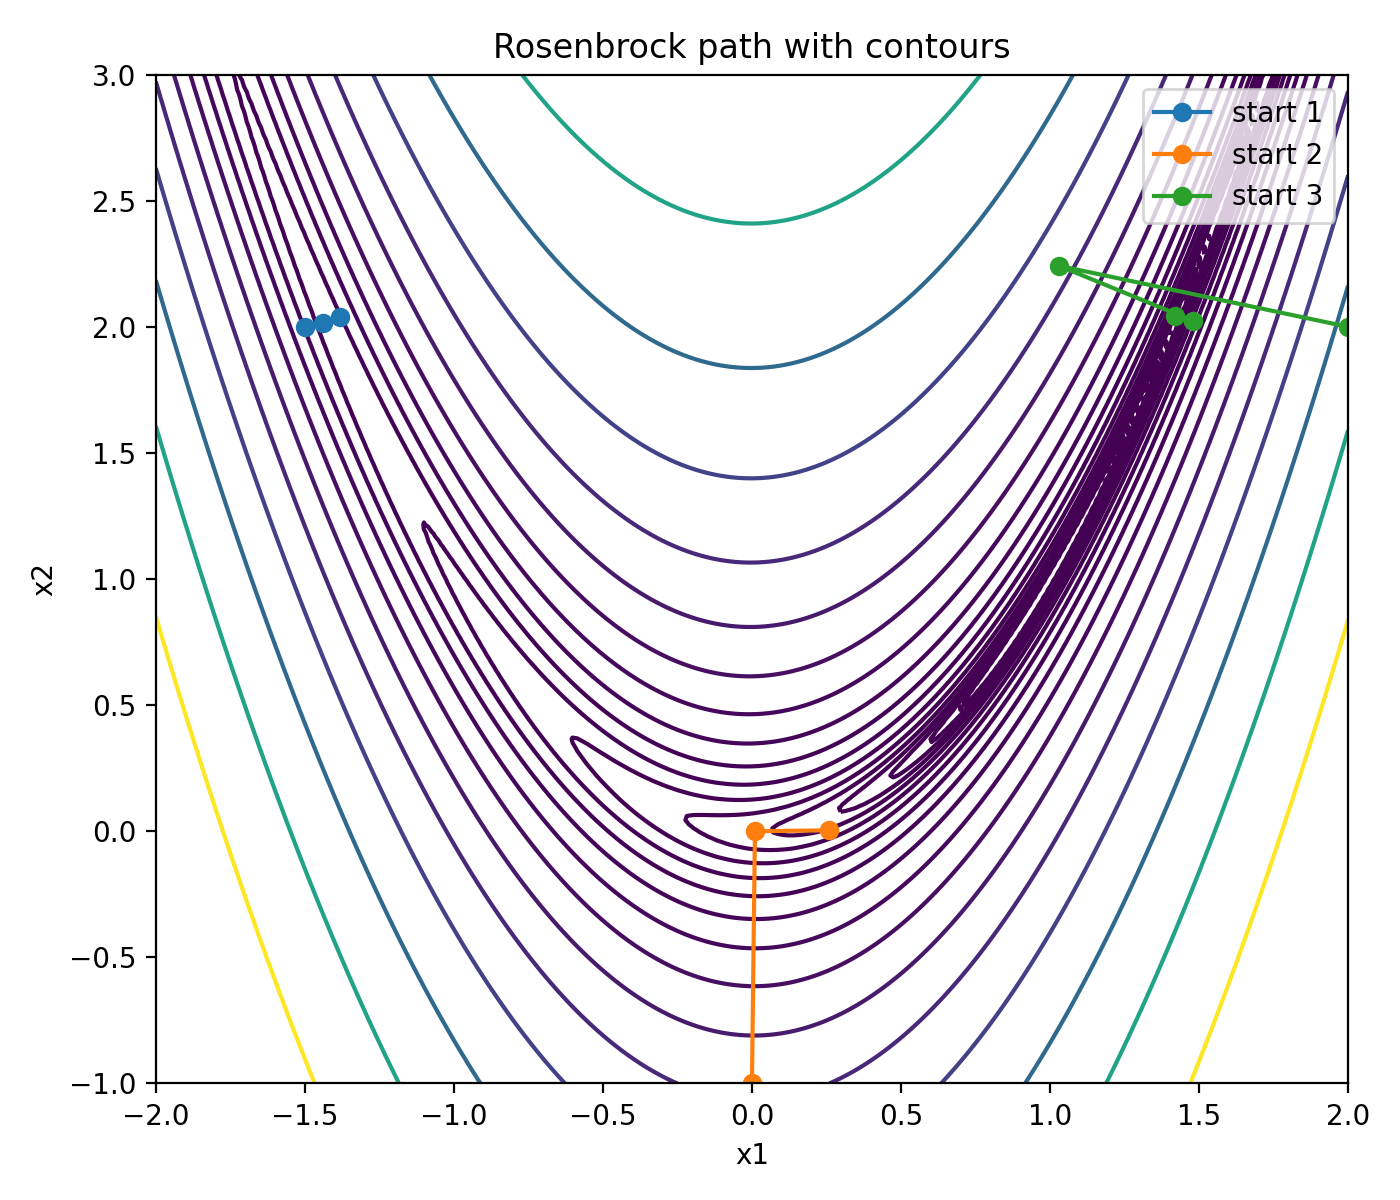
\includegraphics[width=0.8\linewidth]{../readme_plots/rosenbrock_path.png}
    \caption{Optimization paths on Rosenbrock's function from three initial points, overlaid on objective contours.}
\end{figure}

\section*{Convergence Plots}

\begin{figure}[H]
    \centering
    \begin{subfigure}{0.48\linewidth}
        \centering
        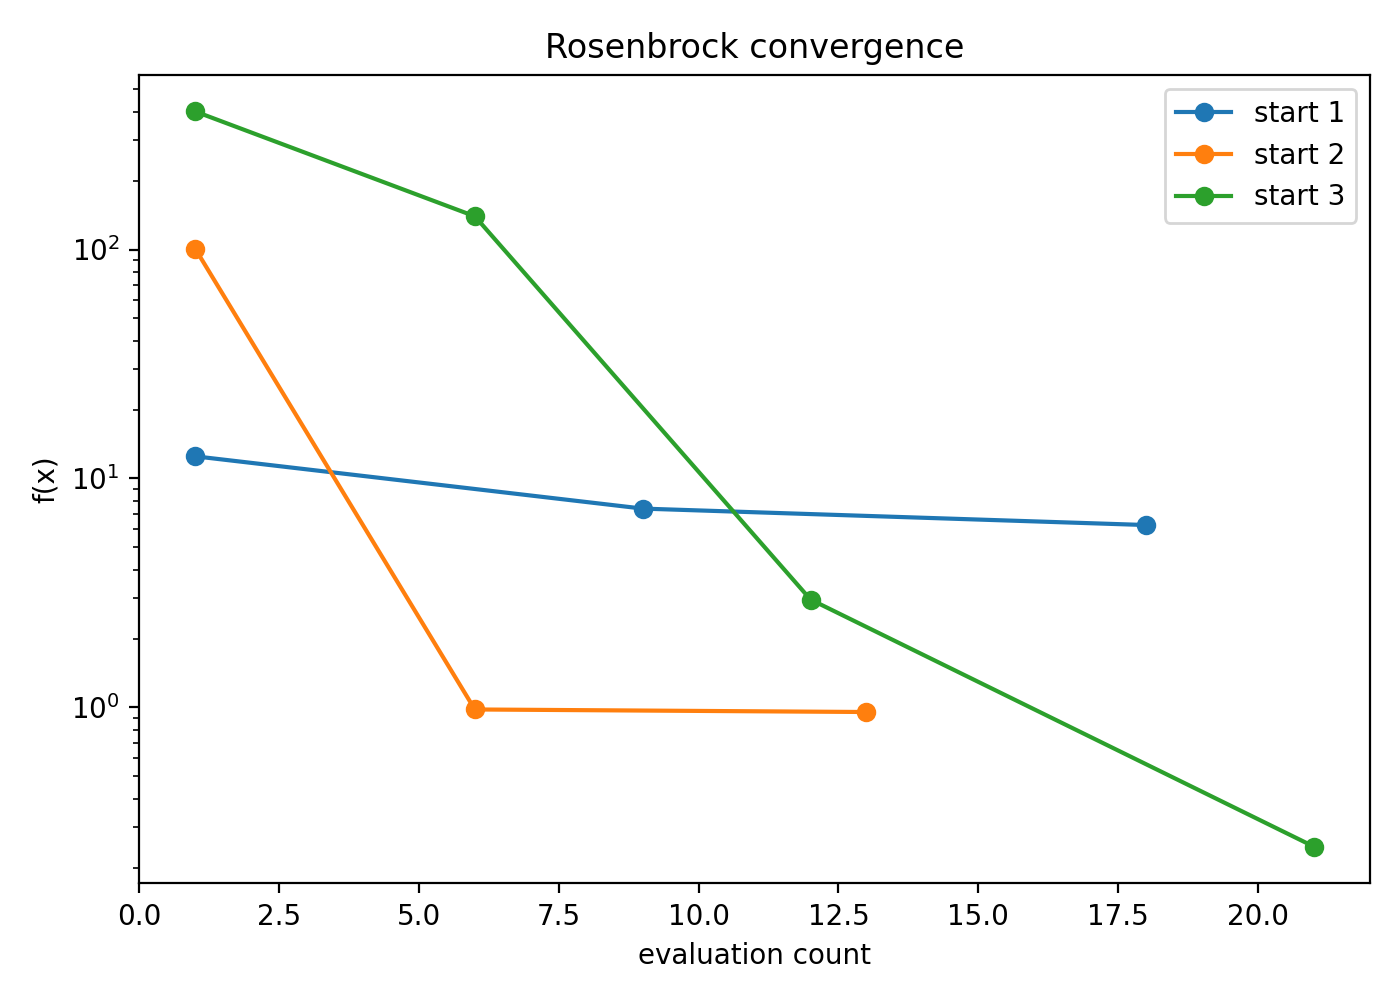
\includegraphics[width=\linewidth]{../readme_plots/simple1_convergence.png}
        \caption{Rosenbrock}
    \end{subfigure}
    \hfill
    \begin{subfigure}{0.48\linewidth}
        \centering
        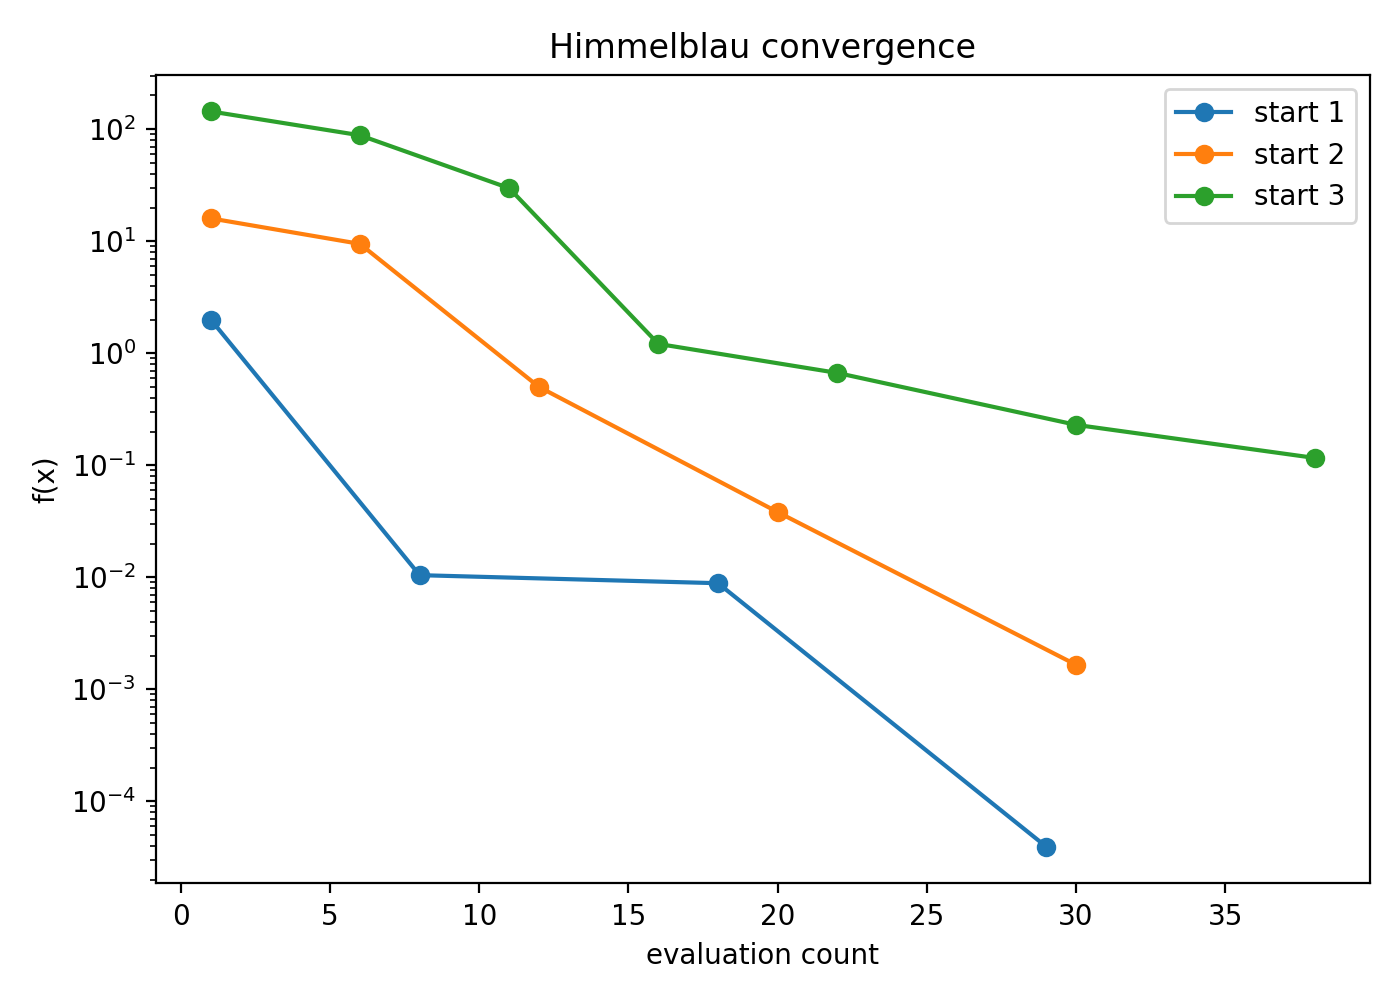
\includegraphics[width=\linewidth]{../readme_plots/simple2_convergence.png}
        \caption{Himmelblau}
    \end{subfigure}

    \vspace{0.75em}

    \begin{subfigure}{0.62\linewidth}
        \centering
        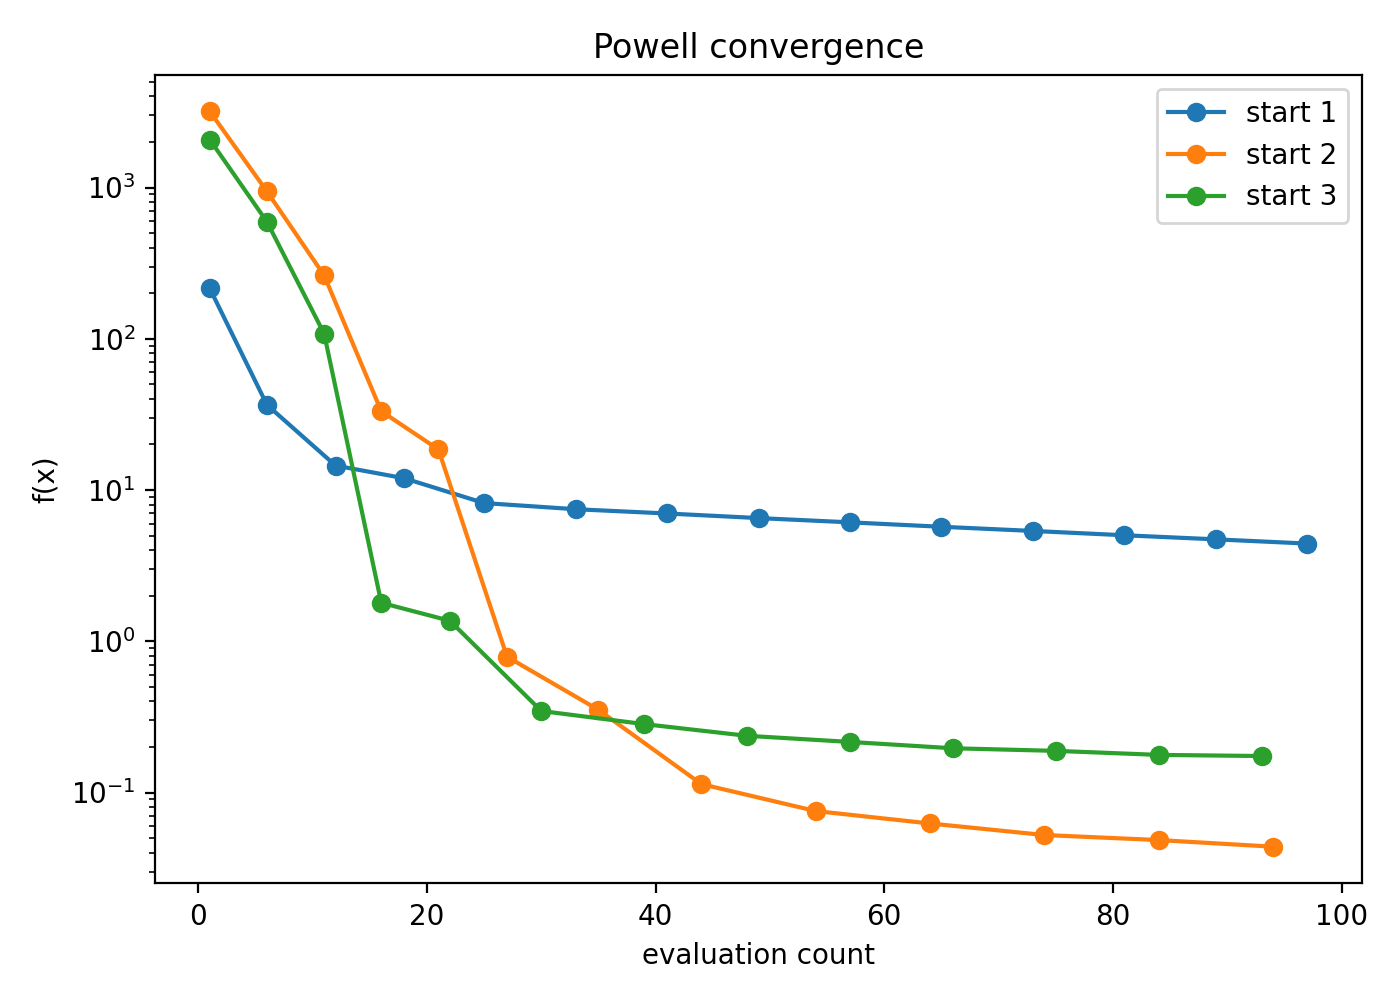
\includegraphics[width=\linewidth]{../readme_plots/simple3_convergence.png}
        \caption{Powell}
    \end{subfigure}
    \caption{Convergence behavior for the three simple optimization problems.}
\end{figure}

\section*{Relevant Code}

\begin{lstlisting}
def descent_step(f, g, x, n, count):
    if count() + 3 > n:
        return x, False

    g_x = g(x)
    f_x = f(x)
    g_norm = np.linalg.norm(g_x)

    if (not np.isfinite(g_norm)) or g_norm == 0.0:
        return x, False

    d = -g_x / g_norm

    alpha = 1.0
    p = 0.5
    beta = 1e-4

    while count() < n:
        x_trial = x + alpha * d
        f_trial = f(x_trial)
        if f_trial <= f_x + beta * alpha * (g_x.T @ d):
            return x_trial, True
        alpha *= p

    return x, False


def optimize(f, g, x0, n, count, prob):
    x_best = x0

    while count() < n:
        x_new, moved = descent_step(f, g, x_best, n, count)
        if not moved:
            break
        x_best = x_new

    return x_best
\end{lstlisting}
